
% [Descrever os produtos a serem gerados, as principais atividades e apresentar um cronograma de trabalho.]



\subsection{Resumo da proposta} % (fold)
\label{sub:resumo_da_proposta}
%[Escrever um resumo da proposta de trabalho do grupo, responder o que será realizado, qual o ponto de partida e realizar conexões com a fundamentação teórica apresentada.]

A utilização de padrões de projeto garantem uma mínima qualidade do software, garantindo maior facilidade na manutenção e evolução do mesmo. Pensando por este lado, a proposta do trabalho da disciplina de Medição e Análise de Software é fazer uma comparação entre a qualidade do software sem a utilização de padrões de projeto e a qualidade do mesmo após a aplicação de padrões. A padronização do software foi feita durante a disciplina de Manutenção e Evolução de Software da Universidade de Brasília.

O ponto de partida para a realização do trabalho serão as medições da qualidade do software sem a utilização de padrões de projeto. Medindo defeitos por linha de código, padronização de código e a cobertura de código. Após o recolhimento de todos os resultados destas medições, serão feitas medições com o mesmo software após a aplicação do mesmo na disciplina de Manutenção e Evolução de software. Com os resultados das duas medições, poderemos compará-los para provar a relação de padrões de projeto e qualidade de software.

O software utilizado nas duas medições será o \textit{GestorPsi}, que é um software de gerência de uma clínica de psicologia. O mesmo foi desenvolvido por alunos da universidade de forma não padronizada e não gerenciada, formando o software de baixa qualidade. Após a utilização do mesmo na disciplina de Manutenção e Evolução de Software, espera-se que o mesmo obtenha uma qualidade, no mínimo, aceitável. A partir das medições realizadas neste trabalhos, poderemos observar se a padronização do software garante melhora na qualidade do mesmo, ou não.

\subsection{Estrutura Analítica do Projeto} % (fold)
\label{sub:estrutura_anal_tica_do_projeto}

% [A Estrutura Analítica de Projetos (EAP), do Inglês, Work breakdown structure (WBS) é uma ferramenta de decomposição do trabalho do projeto em partes manejáveis. É estrutura em árvore, hierárquica (de mais geral para mais específica) orientada às entregas que precisam ser feitas para completar um projeto.
% O objetivo de uma WBS é identificar elementos terminais (os produtos, serviços e resultados a serem feitos em um projeto). Assim, a WBS serve como base para a maior parte do planejamento de projeto.
% A dica de ferramenta a ser utilizada para elaborar a EAP é o XMIND 
% \url{http://www.xmind.net/} ]

\begin{figure}[H]
	\label{eap}
	\centering
	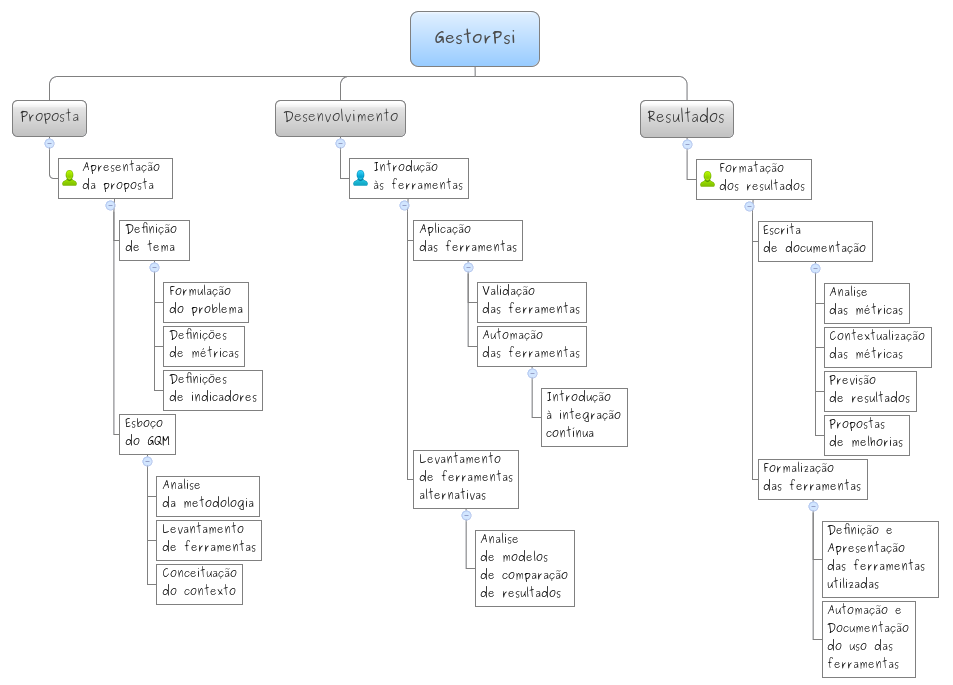
\includegraphics[width=0.8\textwidth]{conteudo/EAP}
	\caption{Estrutura Analítica do Projeto}
\end{figure}


\subsection{Lista de software} % (fold)
\label{sub:lista_de_software}

% [Listar os softwares necessários para o desenvolvimento do projeto]
% Alguns exemplos de ferramentas em http://stackoverflow.com/questions/100298/code-analysis-in-python
Softwares necessários para o desenvolvimento do projeto:
\begin{itemize}
	\item Python 2.7
	\item Django v1.4
	\item Pylint
	\item PyGenie
\end{itemize}

\subsection{Descrição das Atividades} % (fold)
\label{sub:descri_o_das_atividades}

\begin{table}[H]
\centering
\caption{\textbf{Distribuição de atividades}}
\begin{longtable}{|p{4cm}|p{7.5cm}|p{3cm}|}
\hline
\textbf{Atividade} & \textbf{Descrição} & \textbf{Responsáveis} \\ \hline
% A1. Nome da Atividade & Descrição suscinta da atividade & Definir o(s) responsável(is) pela atividade. \\ \hline
A1. Gerar Build & Ambientação, deixar o sistema executável em todas as máquinas, levantar o serviço local e a torná-lo acessível pelo navegador. & \carloss \\ \hline
A2. Análise estática do código. & Utilização da ferramenta de análise estática de código para verificar padrões. & \ziul \\ \hline
A3. Cobertura de código. & Verificar a cobertura de código, registrando a porcentagem de cobertura e o nível dos testes. & \rafael~e \ziul\\ \hline
A4. Verificar coesão e acoplamento do código. & Analisar e registrar o nível de coesão e acoplamento do código. & \carloss \\ \hline
A5. Acompanhar evolução do software. & Acompanhar a evolução do software no decorrer do tempo . & \rafael \\ \hline
\end{longtable}
\label{}
\end{table}


\subsection{Cronograma de Atividades} % (fold)
\label{sub:cronograma_de_atividades}

\begin{table}[H]
\centering
\caption{\textbf{Cronograma de atividades}}
\begin{tabular}{|p{4cm}|p{8cm}|p{2.5cm}|}
\hline
\textbf{Atividade} & \textbf{Descrição} & \textbf{Data} \\ \hline
A1. Gerar Build & Ambientação, deixar o sistema executável em todas as máquinas, levantar o serviço local e a torná-lo acessível pelo navegador. & 23/10/2014 \\ \hline
A2. Análise estática do código. & Utilização da ferramenta de análise estática de código para verificar padrões. & 28/10/2014 \\ \hline
A3. Cobertura de código. & Verificar a cobertura de código, registrando a porcentagem de cobertura e o nível dos testes. & 04/11/2014 \\ \hline
A4. Verificar coesão e acoplamento do código. & Analisar e registrar o nível de coesão e acoplamento do código. & 11/11/2014 \\ \hline
A5. Acompanhar evolução do software. & Acompanhar a evolução do software no decorrer do tempo . & de 16/10/2014 a 27/11/2014 \\ \hline
% Ambiente & Preparar  Estrutura de documentos e diretórios para geração de relatórios & Luiz Oliveira \\ \hline
\end{tabular}
\label{}
\end{table}
